\documentclass[11pt,a4paper]{article}
\usepackage{amsmath}
\usepackage{amssymb}
\usepackage{geometry}
\usepackage{graphicx}
\usepackage{hyperref}
\usepackage{booktabs}
\usepackage{bm}
\usepackage{siunitx}
\usepackage{float}
\usepackage{tikz}
\usetikzlibrary{arrows.meta, positioning, shapes.geometric, calc}

\geometry{margin=1in}

\title{Vehicle Dynamics, Battery, and Sensor Models (Dugoff Tire + Sensor Simulation)}
\author{Mario Tilocca}
\date{January 2026 -- Version 2.1}

\begin{document}


\maketitle


\begin{abstract}
This document presents the transition from a kinematic bicycle model to a dynamic vehicle model incorporating the Dugoff tire model with wheel rotational dynamics. We derive the complete force-based dynamics, normal load distribution with load transfer, slip ratio computation, friction-limited tire forces, wheel angular velocity integration, and Ackermann steering geometry. The hybrid torque-slip model enables realistic simulation of traction limits, wheel spin, wheel lock, and combined longitudinal-lateral dynamics for autonomous mining haul truck applications.
\end{abstract}


\tableofcontents
\clearpage


%=============================================================================
\section{Introduction}
%=============================================================================

\subsection{Motivation for Dynamic Model}

The kinematic bicycle model assumes:
\begin{itemize}
    \item \textbf{No slip:} Pure rolling condition at all times
    \item \textbf{Unlimited traction:} Tire forces can be arbitrarily large
    \item \textbf{Instantaneous response:} No force buildup dynamics
\end{itemize}

These assumptions break down when:
\begin{itemize}
    \item Vehicle operates on low-friction surfaces (gravel, wet haul roads)
    \item Emergency braking or aggressive acceleration
    \item Combined maneuvers (braking while turning)
    \item Realistic traction control and ABS simulation required
\end{itemize}

The Dugoff tire model addresses these by:
\begin{itemize}
    \item Computing friction-limited forces based on normal load
    \item Modeling slip ratios (longitudinal and lateral)
    \item Capturing smooth saturation from linear to sliding regimes
\end{itemize}

\subsection{Model Architecture Evolution}

We present three levels of modeling fidelity:

\textbf{Kinematic Model (V1):}
\begin{equation}
\text{Actuator} \to \text{Drive} \to \text{Velocity} \to \text{Position/Yaw}
\end{equation}

\textbf{Torque-Only Dynamic Model (V2):}
\begin{equation}
\text{Actuator} \to \text{Drive} \to \boxed{\text{Tire Forces (friction-limited)}} \to \text{Acceleration} \to \text{Velocity}
\end{equation}

\textbf{Hybrid Torque-Slip Model (V2.5):}
\begin{equation}
\text{Actuator} \to \boxed{\text{Wheel Dynamics}} \to \boxed{\text{Slip}} \to \boxed{\text{Dugoff Forces}} \to \text{Vehicle Dynamics}
\end{equation}

The hybrid model adds wheel rotational dynamics, enabling natural slip development, wheel spin, and wheel lock simulation.

\subsection{Model Comparison Summary}

\begin{table}[H]
\centering
\begin{tabular}{lccc}
\toprule
\textbf{Feature} & \textbf{Kinematic} & \textbf{Torque-Only} & \textbf{Hybrid} \\
\midrule
Traction limit & Unlimited & $\mu F_z$ & $\mu F_z$ \\
Wheel slip & None & Estimated & Computed \\
Wheel spin & No & No & Yes \\
Wheel lock & No & No & Yes \\
TCS/ABS testing & No & Limited & Full \\
Computational cost & Low & Low & Medium \\
\bottomrule
\end{tabular}
\caption{Tire model comparison}
\end{table}

%=============================================================================
\section{Steering Geometry and Ackermann Model}
\label{sec:steering}
%=============================================================================

\subsection{Virtual Steering Angle}

The bicycle model uses a single \textbf{virtual steering angle} $\delta$ to represent the combined effect of both front wheels. This simplification works well for trajectory planning but requires mapping to individual wheel angles for realistic tire force computation.

\begin{equation}
\delta = \text{virtual steering angle (bicycle model input)}
\end{equation}

The virtual angle corresponds to the steering angle of a hypothetical single front wheel located at the center of the front axle.

\subsection{Ackermann Steering Geometry}

For a vehicle turning with radius $R$, all wheels must have their axes intersect at a common point (the Instantaneous Center of Rotation, ICR) to achieve pure rolling without tire scrub.

\begin{figure}[H]
\centering
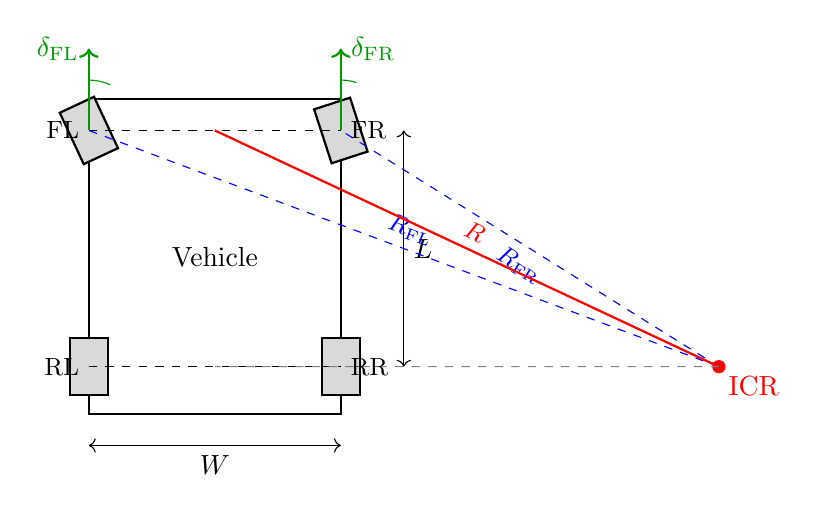
\begin{tikzpicture}[scale=0.8]
    % Vehicle body
    \draw[thick] (-2, 0) rectangle (2, 5);
    
    % Wheels
    \draw[thick, fill=gray!30] (-2.3, 0.3) rectangle (-1.7, 1.2);  % RL
    \draw[thick, fill=gray!30] (1.7, 0.3) rectangle (2.3, 1.2);    % RR
    
    % Front wheels (rotated for steering)
    \begin{scope}[shift={(-2, 4.5)}, rotate=25]
        \draw[thick, fill=gray!30] (-0.3, -0.45) rectangle (0.3, 0.45);
    \end{scope}
    \begin{scope}[shift={(2, 4.5)}, rotate=18]
        \draw[thick, fill=gray!30] (-0.3, -0.45) rectangle (0.3, 0.45);
    \end{scope}
    
    % Axles
    \draw[dashed] (-2, 0.75) -- (2, 0.75);
    \draw[dashed] (-2, 4.5) -- (2, 4.5);
    
    % Wheelbase dimension
    \draw[<->] (3, 0.75) -- (3, 4.5) node[midway, right] {$L$};
    
    % Track width dimension
    \draw[<->] (-2, -0.5) -- (2, -0.5) node[midway, below] {$W$};
    
    % Turn center (ICR)
    \coordinate (ICR) at (8, 0.75);
    \fill[red] (ICR) circle (3pt) node[below right] {ICR};
    
    % Turn radii
    \draw[blue, dashed] (ICR) -- (-2, 4.5) node[midway, above, sloped, font=\small] {$R_{\text{FL}}$};
    \draw[blue, dashed] (ICR) -- (2, 4.5) node[midway, below, sloped, font=\small] {$R_{\text{FR}}$};
    \draw[red, thick] (ICR) -- (0, 4.5) node[midway, above, sloped, font=\small] {$R$};
    \draw[gray, dashed] (ICR) -- (0, 0.75);
    
    % Steering angles
    \draw[green!60!black, thick, ->] (-2, 4.5) -- (-2, 5.8) node[left] {$\delta_{\text{FL}}$};
    \draw[green!60!black, thick, ->] (2, 4.5) -- (2, 5.8) node[right] {$\delta_{\text{FR}}$};
    
    % Angle arcs
    \draw[green!60!black] (-2, 5.3) arc (90:65:0.8);
    \draw[green!60!black] (2, 5.3) arc (90:72:0.8);
    
    % Labels
    \node at (0, 2.5) {Vehicle};
    \node[font=\small] at (-2, 4.5) [left] {FL};
    \node[font=\small] at (2, 4.5) [right] {FR};
    \node[font=\small] at (-2, 0.75) [left] {RL};
    \node[font=\small] at (2, 0.75) [right] {RR};
    
\end{tikzpicture}
\caption{Ackermann steering geometry showing inner wheel (FR) turning more than outer wheel (FL) for a right turn}
\label{fig:ackermann}
\end{figure}

\subsection{Ackermann Equations}

\textbf{Turn radius from virtual steering angle:}
\begin{equation}
\boxed{R = \frac{L}{\tan(\delta)}}
\label{eq:turn_radius}
\end{equation}

where:
\begin{itemize}
    \item $R$ -- turn radius from rear axle center to ICR (m)
    \item $L$ -- wheelbase (m)
    \item $\delta$ -- virtual steering angle (rad)
\end{itemize}

\textbf{Per-wheel turn radii:}

For a right turn ($\delta > 0$), the turn center is to the right of the vehicle:
\begin{align}
R_{\text{FL}} &= R + \frac{W}{2} \quad \text{(outer wheel, larger radius)} \\
R_{\text{FR}} &= R - \frac{W}{2} \quad \text{(inner wheel, smaller radius)}
\end{align}

where $W$ is the track width (m).

\textbf{Individual wheel steering angles:}
\begin{align}
\boxed{\delta_{\text{FL}} = \arctan\left(\frac{L}{R + W/2}\right)} \label{eq:delta_fl} \\
\boxed{\delta_{\text{FR}} = \arctan\left(\frac{L}{R - W/2}\right)} \label{eq:delta_fr}
\end{align}

\textbf{Key property:} For a right turn, the inner wheel (FR) turns \textit{more} than the outer wheel (FL):
\begin{equation}
|\delta_{\text{FR}}| > |\delta_{\text{FL}}| \quad \text{when } \delta > 0
\end{equation}

This ensures all wheel axes intersect at the ICR, minimizing tire scrub.

\subsection{Ackermann Condition}

The classic Ackermann condition states:
\begin{equation}
\boxed{\cot(\delta_{\text{outer}}) - \cot(\delta_{\text{inner}}) = \frac{W}{L}}
\label{eq:ackermann_condition}
\end{equation}

\textbf{Proof:} From the geometry:
\begin{align}
\cot(\delta_{\text{FL}}) &= \frac{R + W/2}{L} \\
\cot(\delta_{\text{FR}}) &= \frac{R - W/2}{L} \\
\cot(\delta_{\text{FL}}) - \cot(\delta_{\text{FR}}) &= \frac{(R + W/2) - (R - W/2)}{L} = \frac{W}{L} \quad \square
\end{align}

This condition is independent of turn radius $R$ and depends only on vehicle geometry.

\subsection{Ackermann Percentage}

Real vehicles rarely use perfect (100\%) Ackermann geometry. A partial Ackermann configuration blends between:
\begin{itemize}
    \item \textbf{Full Ackermann (100\%):} $\delta_{\text{FL}} \neq \delta_{\text{FR}}$ as derived above
    \item \textbf{Parallel steering (0\%):} $\delta_{\text{FL}} = \delta_{\text{FR}} = \delta$
\end{itemize}

The Ackermann percentage $\alpha_{\text{ack}} \in [0, 1]$ controls the blend:
\begin{align}
\delta_{\text{FL}} &= \alpha_{\text{ack}} \cdot \delta_{\text{FL,Ackermann}} + (1 - \alpha_{\text{ack}}) \cdot \delta \\
\delta_{\text{FR}} &= \alpha_{\text{ack}} \cdot \delta_{\text{FR,Ackermann}} + (1 - \alpha_{\text{ack}}) \cdot \delta
\end{align}

\textbf{Typical values:}
\begin{itemize}
    \item Passenger cars: $\alpha_{\text{ack}} = 0.80 - 0.90$ (compromise for tire wear at speed)
    \item Racing vehicles: $\alpha_{\text{ack}} = 0.50 - 0.70$ (optimized for cornering)
    \item Mining trucks: $\alpha_{\text{ack}} = 0.95 - 1.00$ (low-speed maneuverability)
\end{itemize}

\subsection{Speed-Dependent Steering Limit}

At high speeds, large steering angles cause excessive lateral acceleration and potential rollover. A speed-dependent limit reduces maximum steering:

\begin{equation}
\delta_{\max}(v) = \delta_{\max,0} \cdot r(v)
\end{equation}

where the reduction factor $r(v)$ is:
\begin{equation}
\boxed{r(v) = \begin{cases}
1 & v \leq v_{\text{start}} \\
1 - (1 - r_{\text{high}}) \cdot \dfrac{v - v_{\text{start}}}{v_{\text{end}} - v_{\text{start}}} & v_{\text{start}} < v < v_{\text{end}} \\
r_{\text{high}} & v \geq v_{\text{end}}
\end{cases}}
\label{eq:speed_steering_limit}
\end{equation}

\textbf{Parameters:}
\begin{itemize}
    \item $\delta_{\max,0}$ -- maximum steering angle at low speed (rad)
    \item $v_{\text{start}}$ -- speed at which limiting begins (m/s)
    \item $v_{\text{end}}$ -- speed at which full limiting is applied (m/s)
    \item $r_{\text{high}}$ -- reduction ratio at high speed (e.g., 0.35 = 35\% of max)
\end{itemize}

\textbf{Example for Heavy-Duty Electric Vehicle:}
\begin{align}
\delta_{\max,0} &= 35° \\
v_{\text{start}} &= 8 \text{ m/s} \\
v_{\text{end}} &= 25 \text{ m/s} \\
r_{\text{high}} &= 0.35
\end{align}

At 25 m/s (90 km/h), maximum steering is limited to $35° \times 0.35 = 12.25°$.

\subsection{Steering Rate Limiting}

Physical steering systems have bandwidth limitations due to hydraulic flow (mining trucks) or electric motor limits (passenger cars):

\begin{equation}
\boxed{\dot{\delta} = \text{clamp}\left(\frac{\delta_{\text{cmd}} - \delta}{\Delta t}, -\dot{\delta}_{\max}, +\dot{\delta}_{\max}\right)}
\label{eq:rate_limit}
\end{equation}

\textbf{Typical maximum steering rates:}
\begin{itemize}
    \item Passenger cars (electric): $\dot{\delta}_{\max} = 400 - 600$ °/s
    \item Mining trucks (hydraulic): $\dot{\delta}_{\max} = 30 - 60$ °/s
\end{itemize}

The discrete-time update becomes:
\begin{equation}
\delta[k+1] = \delta[k] + \text{clamp}\left(\delta_{\text{des}} - \delta[k], -\dot{\delta}_{\max} \Delta t, +\dot{\delta}_{\max} \Delta t\right)
\end{equation}

\subsection{Minimum Turn Radius}

At maximum steering angle, the minimum turn radius is:
\begin{equation}
R_{\min} = \frac{L}{\tan(\delta_{\max})}
\end{equation}

For Heavy-Duty Electric Vehicle with $L = 6.3$ m and $\delta_{\max} = 35°$:
\begin{equation}
R_{\min} = \frac{6.3}{\tan(35°)} = \frac{6.3}{0.700} = 9.0 \text{ m}
\end{equation}

The inner wheel turn radius is:
\begin{equation}
R_{\text{inner}} = R_{\min} - \frac{W}{2} = 9.0 - 2.0 = 7.0 \text{ m}
\end{equation}

This determines the minimum pit road width for U-turns.

\subsection{Steering System Block Diagram}

\begin{figure}[H]
\centering
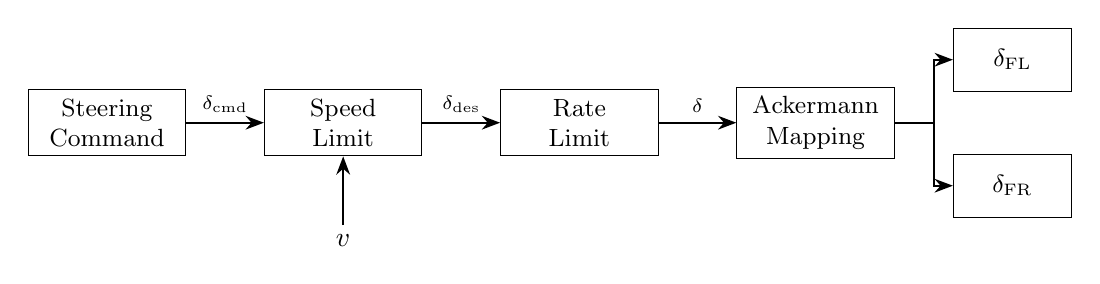
\begin{tikzpicture}[
    block/.style={rectangle, draw, minimum width=2.0cm, minimum height=0.8cm, align=center, font=\small},
    arrow/.style={-{Stealth[scale=1.0]}, thick}
]

% Blocks
\node[block] (cmd) at (0, 0) {Steering\\Command};
\node[block] (limit) at (3, 0) {Speed\\Limit};
\node[block] (rate) at (6, 0) {Rate\\Limit};
\node[block] (acker) at (9, 0) {Ackermann\\Mapping};

% Outputs
\node[block, minimum width=1.5cm] (fl) at (11.5, 0.8) {$\delta_{\text{FL}}$};
\node[block, minimum width=1.5cm] (fr) at (11.5, -0.8) {$\delta_{\text{FR}}$};

% Speed input
\node (speed) at (3, -1.5) {$v$};

% Arrows
\draw[arrow] (cmd) -- (limit) node[midway, above, font=\scriptsize] {$\delta_{\text{cmd}}$};
\draw[arrow] (limit) -- (rate) node[midway, above, font=\scriptsize] {$\delta_{\text{des}}$};
\draw[arrow] (rate) -- (acker) node[midway, above, font=\scriptsize] {$\delta$};
\draw[arrow] (acker.east) -- ++(0.5, 0) |- (fl.west);
\draw[arrow] (acker.east) -- ++(0.5, 0) |- (fr.west);
\draw[arrow] (speed) -- (limit);

\end{tikzpicture}
\caption{Steering system signal flow}
\label{fig:steering_block}
\end{figure}

%=============================================================================
\section{Force-Based Longitudinal Dynamics}
%=============================================================================

\subsection{Equations of Motion}

Newton's second law in the longitudinal direction:
\begin{equation}
m \frac{dv}{dt} = \sum F_x - F_{\text{drag}} - F_{\text{roll}}
\end{equation}

where:
\begin{align}
\sum F_x &= F_{x,\text{fl}} + F_{x,\text{fr}} + F_{x,\text{rl}} + F_{x,\text{rr}} \quad \text{(sum of tire forces)} \\
F_{\text{drag}} &= \frac{1}{2} \rho C_d A v^2 \\
F_{\text{roll}} &= C_{\text{roll}} \cdot \text{sgn}(v)
\end{align}

\subsection{Tire Force Allocation}

For a rear-wheel-drive vehicle:
\begin{align}
F_{x,\text{fl}} &= 0 \quad \text{(front wheels: unpowered)} \\
F_{x,\text{fr}} &= 0 \\
F_{x,\text{rl}} &= f_{\text{Dugoff}}(\sigma_{x,\text{rl}}, \sigma_{y,\text{rl}}, F_{z,\text{rl}}) \\
F_{x,\text{rr}} &= f_{\text{Dugoff}}(\sigma_{x,\text{rr}}, \sigma_{y,\text{rr}}, F_{z,\text{rr}})
\end{align}

where $f_{\text{Dugoff}}$ is the tire model function (detailed in Section~\ref{sec:dugoff}).

%=============================================================================
\section{Normal Load Distribution}
%=============================================================================

\subsection{Static Load Distribution}

Weight distribution between front and rear axles:
\begin{align}
F_{z,\text{front}}^{\text{static}} &= \frac{mg \cdot L_r}{L} \\
F_{z,\text{rear}}^{\text{static}} &= \frac{mg \cdot L_f}{L}
\end{align}

where:
\begin{itemize}
    \item $m$ -- vehicle mass (kg)
    \item $g = 9.81$ m/s$^2$ -- gravitational acceleration
    \item $L = L_f + L_r$ -- wheelbase (m)
    \item $L_f$ -- distance from CoG to front axle (m)
    \item $L_r$ -- distance from CoG to rear axle (m)
\end{itemize}

\subsection{Longitudinal Load Transfer}

During acceleration or braking, normal load shifts between axles:
\begin{equation}
\boxed{\Delta F_z = \frac{m \cdot a_x \cdot h_{\text{cg}}}{L}}
\end{equation}

where:
\begin{itemize}
    \item $a_x$ -- longitudinal acceleration (m/s$^2$), positive = acceleration
    \item $h_{\text{cg}}$ -- center of gravity height (m)
\end{itemize}

\textbf{Dynamic normal loads:}
\begin{align}
F_{z,\text{front}} &= F_{z,\text{front}}^{\text{static}} - \Delta F_z \\
F_{z,\text{rear}} &= F_{z,\text{rear}}^{\text{static}} + \Delta F_z
\end{align}

\textbf{Physical interpretation:}
\begin{itemize}
    \item $a_x > 0$ (acceleration): Weight transfers to rear $\Rightarrow$ more rear traction
    \item $a_x < 0$ (braking): Weight transfers to front $\Rightarrow$ more front braking capacity
\end{itemize}

\subsection{Lateral Load Transfer}

During cornering with lateral acceleration $a_y$:
\begin{equation}
\Delta F_{z,\text{lat}} = \frac{m \cdot a_y \cdot h_{\text{cg}}}{W}
\end{equation}

where $W$ is the track width (m).

\subsection{Per-Wheel Normal Loads}

Combined longitudinal and lateral load transfer:
\begin{align}
F_{z,\text{fl}} &= \frac{1}{2}\left( F_{z,\text{front}} - \Delta F_{z,\text{lat,front}} \right) \\
F_{z,\text{fr}} &= \frac{1}{2}\left( F_{z,\text{front}} + \Delta F_{z,\text{lat,front}} \right) \\
F_{z,\text{rl}} &= \frac{1}{2}\left( F_{z,\text{rear}} - \Delta F_{z,\text{lat,rear}} \right) \\
F_{z,\text{rr}} &= \frac{1}{2}\left( F_{z,\text{rear}} + \Delta F_{z,\text{lat,rear}} \right)
\end{align}

\subsection{Example: Heavy-Duty Electric Vehicle Mining Truck}

\textbf{Parameters:}
\begin{align}
m &= 218{,}000 \text{ kg (empty)} \\
L &= 6.3 \text{ m} \\
h_{\text{cg}} &= 2.8 \text{ m} \\
L_f &= 2.52 \text{ m (40\% of wheelbase)} \\
L_r &= 3.78 \text{ m (60\% of wheelbase)}
\end{align}

\textbf{Static loads:}
\begin{align}
F_{z,\text{front}}^{\text{static}} &= \frac{218{,}000 \times 9.81 \times 3.78}{6.3} = 1{,}284{,}000 \text{ N} \\
F_{z,\text{rear}}^{\text{static}} &= \frac{218{,}000 \times 9.81 \times 2.52}{6.3} = 856{,}000 \text{ N}
\end{align}

\textbf{Load transfer during braking at $a_x = -2.0$ m/s$^2$:}
\begin{align}
\Delta F_z &= \frac{218{,}000 \times (-2.0) \times 2.8}{6.3} = -193{,}600 \text{ N} \\
F_{z,\text{front}} &= 1{,}284{,}000 + 193{,}600 = 1{,}478{,}000 \text{ N} \\
F_{z,\text{rear}} &= 856{,}000 - 193{,}600 = 662{,}000 \text{ N}
\end{align}

Result: Front axle load increases by 15\%, rear decreases by 23\% during braking.

%=============================================================================
\section{Dugoff Tire Model}
\label{sec:dugoff}
%=============================================================================

\subsection{Fundamental Equations}

Tire forces are given by:
\begin{align}
\boxed{F_x = C_x \sigma_x f(\lambda)} \label{eq:Fx_dugoff}\\
\boxed{F_y = C_y \sigma_y f(\lambda)} \label{eq:Fy_dugoff}
\end{align}

where:
\begin{itemize}
    \item $F_x, F_y$ -- longitudinal and lateral tire forces (N)
    \item $C_x, C_y$ -- slip stiffness coefficients (N), load-dependent
    \item $\sigma_x, \sigma_y$ -- longitudinal and lateral slip ratios
    \item $f(\lambda)$ -- friction saturation function
    \item $\lambda$ -- friction utilization parameter
\end{itemize}

\subsection{Slip Ratios}

\textbf{Longitudinal slip ratio:}
\begin{equation}
\boxed{\sigma_x = \frac{\omega R - V_x}{\max(|V_x|, |\omega R|, V_{\min})}}
\label{eq:slip_ratio}
\end{equation}

where:
\begin{itemize}
    \item $\omega$ -- wheel angular velocity (rad/s)
    \item $R$ -- tire effective radius (m)
    \item $V_x$ -- vehicle longitudinal velocity (m/s)
    \item $V_{\min} \approx 0.1$ m/s -- prevents division by zero
\end{itemize}

\textbf{Sign convention:}
\begin{align}
\sigma_x > 0 &\quad \text{Driving (wheel faster than vehicle)} \\
\sigma_x < 0 &\quad \text{Braking (wheel slower than vehicle)} \\
\sigma_x = 0 &\quad \text{Free rolling}
\end{align}

\textbf{Lateral slip ratio:}
\begin{equation}
\sigma_y = \frac{V_y}{V_x} \approx \tan(\alpha) \approx \alpha
\end{equation}

where $\alpha$ is tire slip angle (rad), valid for small angles ($|\alpha| < 0.2$ rad).

\subsection{Load-Dependent Slip Stiffness}

Tire stiffness scales with normal load:
\begin{align}
C_x(F_z) &= C_{x,\text{base}} \cdot \frac{F_z}{F_{z,\text{ref}}} \\
C_y(F_z) &= C_{y,\text{base}} \cdot \frac{F_z}{F_{z,\text{ref}}}
\end{align}

where:
\begin{itemize}
    \item $C_{x,\text{base}}, C_{y,\text{base}}$ -- baseline stiffness at reference load (N)
    \item $F_{z,\text{ref}}$ -- reference normal load (N)
\end{itemize}

Typical values for mining truck tires:
\begin{itemize}
    \item $C_{x,\text{base}} \approx 280{,}000$ N
    \item $C_{y,\text{base}} \approx 220{,}000$ N
    \item $F_{z,\text{ref}} = 100{,}000$ N
\end{itemize}

\subsection{Friction Utilization Parameter}

The key parameter governing saturation:
\begin{equation}
\boxed{\lambda = \frac{\mu F_z}{2\sqrt{(C_x \sigma_x)^2 + (C_y \sigma_y)^2}}}
\label{eq:lambda}
\end{equation}

where $\mu$ is the coefficient of friction (surface-dependent).

\textbf{Physical interpretation:}
\begin{align}
\lambda \geq 1 &\quad \text{Linear regime (tire not saturated)} \\
\lambda < 1 &\quad \text{Nonlinear regime (friction-limited, sliding)}
\end{align}

\subsection{Friction Saturation Function}

\begin{equation}
\boxed{f(\lambda) = \begin{cases}
(2 - \lambda)\lambda, & \lambda < 1 \\
1, & \lambda \geq 1
\end{cases}}
\label{eq:saturation}
\end{equation}

\textbf{Properties:}
\begin{itemize}
    \item Continuous at $\lambda = 1$: $\lim_{\lambda \to 1^-} f(\lambda) = 1$
    \item Smooth transition from linear to saturated regime
    \item Maximum value: $f_{\max} = 1$ at $\lambda = 1$
\end{itemize}

\subsection{Friction Circle Constraint}

\textbf{Theorem:} The total tire force never exceeds the friction limit:
\begin{equation}
\sqrt{F_x^2 + F_y^2} \leq \mu F_z
\end{equation}

\textbf{Proof:} For $\lambda < 1$ (friction-limited case):
\begin{align}
\sqrt{F_x^2 + F_y^2} &= \sqrt{(C_x \sigma_x f)^2 + (C_y \sigma_y f)^2} \\
&= f(\lambda) \sqrt{C_x^2 \sigma_x^2 + C_y^2 \sigma_y^2} \\
&= (2\lambda - \lambda^2) \cdot \frac{\mu F_z}{2\lambda} \quad \text{(from definition of $\lambda$)} \\
&= \left(1 - \frac{\lambda}{2}\right) \mu F_z \\
&< \mu F_z \quad \text{(since } 0 < \lambda < 1\text{)} \quad \square
\end{align}

\subsection{Slip-Force Characteristic Curve}

The Dugoff model produces the characteristic slip-force curve:

\begin{figure}[H]
\centering
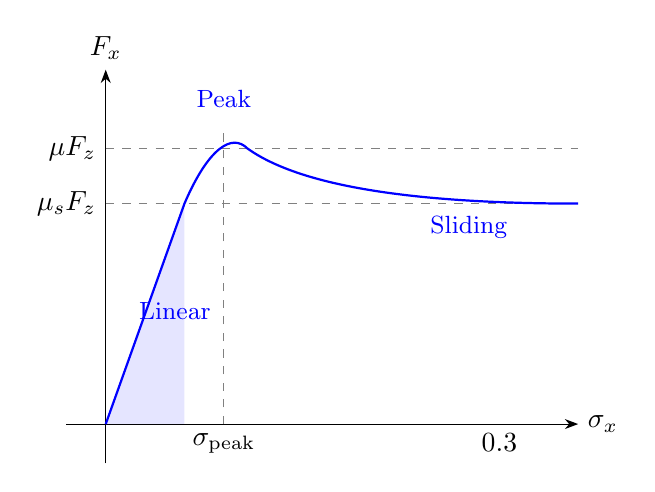
\begin{tikzpicture}[scale=1.0]
    % Axes
    \draw[-{Stealth}] (-0.5, 0) -- (6, 0) node[right] {$\sigma_x$};
    \draw[-{Stealth}] (0, -0.5) -- (0, 4.5) node[above] {$F_x$};
    
    % Labels on axes
    \node[below] at (1.5, 0) {$\sigma_{\text{peak}}$};
    \node[below] at (5, 0) {0.3};
    \node[left] at (0, 3.5) {$\mu F_z$};
    \node[left] at (0, 2.8) {$\mu_s F_z$};
    
    % Reference lines
    \draw[dashed, gray] (0, 3.5) -- (6, 3.5);
    \draw[dashed, gray] (0, 2.8) -- (6, 2.8);
    \draw[dashed, gray] (1.5, 0) -- (1.5, 3.7);
    
    % Dugoff curve
    \draw[thick, blue] (0, 0) -- (1.0, 2.8) 
        .. controls (1.3, 3.5) and (1.6, 3.7) .. (1.8, 3.5)
        .. controls (2.5, 3.0) and (4.0, 2.8) .. (6, 2.8);
    
    % Annotations
    \node[blue, above right] at (0.3, 1.2) {\small Linear};
    \node[blue, above] at (1.5, 3.9) {\small Peak};
    \node[blue, right] at (4.0, 2.5) {\small Sliding};
    
    % Fill linear region
    \fill[blue, opacity=0.1] (0, 0) -- (1.0, 2.8) -- (1.0, 0) -- cycle;
    
\end{tikzpicture}
\caption{Dugoff slip-force characteristic showing linear region, peak grip, and sliding region}
\label{fig:slip_force}
\end{figure}

%=============================================================================
\section{Wheel Rotational Dynamics}
\label{sec:wheel_dynamics}
%=============================================================================

This section introduces the key addition for the hybrid model: independent wheel speed integration.

\subsection{Motivation}

In the torque-only model, wheel speed is derived from vehicle speed:
\begin{equation}
\omega = \frac{V_x}{R} \quad \Rightarrow \quad \sigma_x = 0 \text{ always!}
\end{equation}

This prevents modeling of:
\begin{itemize}
    \item Wheel spin during aggressive acceleration
    \item Wheel lock during hard braking
    \item Natural slip development
    \item TCS/ABS algorithm testing
\end{itemize}

The solution is to integrate wheel angular velocity independently.

\subsection{Single Wheel Free Body Diagram}

For each wheel, applying Newton's second law for rotation:

\begin{equation}
\boxed{I_w \dot{\omega} = \tau_{\text{drive}} - \tau_{\text{brake}} - F_x \cdot R}
\label{eq:wheel_dynamics}
\end{equation}

where:
\begin{itemize}
    \item $I_w$ = wheel rotational inertia (kg$\cdot$m$^2$)
    \item $\omega$ = wheel angular velocity (rad/s)
    \item $\dot{\omega}$ = wheel angular acceleration (rad/s$^2$)
    \item $\tau_{\text{drive}}$ = drive torque at wheel (N$\cdot$m)
    \item $\tau_{\text{brake}}$ = brake torque (N$\cdot$m), always $\geq 0$
    \item $F_x$ = longitudinal tire force from Dugoff (N)
    \item $R$ = tire effective rolling radius (m)
\end{itemize}

\subsection{Drive Torque Distribution}

For a rear-wheel drive (RWD) configuration:

\begin{equation}
\tau_{\text{drive,rl}} = \tau_{\text{drive,rr}} = \frac{\tau_{\text{motor}} \cdot N_{\text{gear}} \cdot \eta_{\text{drivetrain}}}{2}
\end{equation}

\begin{equation}
\tau_{\text{drive,fl}} = \tau_{\text{drive,fr}} = 0 \quad \text{(front wheels not driven)}
\end{equation}

where:
\begin{itemize}
    \item $\tau_{\text{motor}}$ = motor shaft torque (N$\cdot$m)
    \item $N_{\text{gear}}$ = final drive gear ratio (dimensionless)
    \item $\eta_{\text{drivetrain}}$ = drivetrain efficiency (typically 0.90-0.95)
\end{itemize}

\subsection{Brake Torque Distribution}

Brake torque is distributed with a front/rear bias:

\begin{align}
\tau_{\text{brake,fl}} = \tau_{\text{brake,fr}} &= \frac{\tau_{\text{brake,total}} \cdot \beta_{\text{front}}}{2} \\
\tau_{\text{brake,rl}} = \tau_{\text{brake,rr}} &= \frac{\tau_{\text{brake,total}} \cdot (1 - \beta_{\text{front}})}{2}
\end{align}

where $\beta_{\text{front}}$ is the front brake bias (typically 0.40-0.60).

For mining trucks with rear weight bias: $\beta_{\text{front}} = 0.40$ (40\% front, 60\% rear).

\subsection{Wheel Inertia}

The wheel rotational inertia includes:
\begin{equation}
I_w = I_{\text{tire}} + I_{\text{rim}} + I_{\text{brake}} + I_{\text{hub}}
\end{equation}

Typical values:
\begin{itemize}
    \item Passenger car: $I_w \approx 1.5-3.0$ kg$\cdot$m$^2$
    \item Mining haul truck (Heavy-Duty Electric Vehicle): $I_w \approx 800-1500$ kg$\cdot$m$^2$
\end{itemize}

\subsection{Discrete-Time Integration}

Using forward Euler integration:

\begin{equation}
\omega[k+1] = \omega[k] + \frac{\Delta t}{I_w} \left( \tau_{\text{drive}} - \tau_{\text{brake}} \cdot \text{sgn}(\omega[k]) - F_x[k] \cdot R \right)
\label{eq:wheel_integration}
\end{equation}

\textbf{Wheel Lock Detection:}
\begin{equation}
\text{if } \omega[k] > 0 \text{ and } \omega[k+1] < 0 \text{ and } \tau_{\text{brake}} > 0: \quad \omega[k+1] = 0
\end{equation}

This prevents non-physical sign reversal during braking.

\subsection{Stability Criterion}

The explicit integration is stable when:
\begin{equation}
\Delta t < \frac{2 I_w}{C_x R^2}
\end{equation}

For Heavy-Duty Electric Vehicle parameters ($I_w = 1000$ kg$\cdot$m$^2$, $C_x = 280{,}000$ N, $R = 1.93$ m):
\begin{equation}
\Delta t_{\max} \approx \frac{2 \times 1000}{280{,}000 \times 1.93^2} \approx 1.9 \text{ ms}
\end{equation}

Simulation timestep of 1 ms provides adequate stability margin.

%=============================================================================


% -------------------- Added from Sensor/Kinematics document (Sections 6-11) --------------------

\section{Battery and Energy Model}
\label{sec:battery}

This section documents the battery state and power-flow logic as implemented in \texttt{BatteryPlant} and used by the drivetrain/drive subsystem.

\subsection{State Variables}
The battery plant tracks:
\begin{itemize}
    \item State of charge: $\mathrm{SOC} \in [0,1]$
    \item Terminal voltage: $V$ (V)
    \item Current: $I$ (A), with the convention $I>0$ = discharge, $I<0$ = charge (regen)
    \item Electrical power: $P$ (W), with $P>0$ = discharge, $P<0$ = charge
\end{itemize}

\subsection{Open-Circuit Voltage (SOC-Dependent)}
A simple SOC-dependent voltage model is used (updated \emph{before} computing current):
\begin{equation}
V(\mathrm{SOC}) = V_{\text{nom}} \left(0.85 + 0.30\,\mathrm{SOC}\right)
\label{eq:batt_voltage_soc}
\end{equation}
with $V_{\text{nom}} = 400$ V. This yields $340$ V at $0\%$ SOC, $400$ V at $50\%$, and $460$ V at $100\%$.

\subsection{Power Clamping to Motor Limits}
The battery plant receives an electrical power demand (from the drive plant). This demand is clamped to the motor power capability:
\begin{equation}
P_{\text{dem}} \leftarrow \mathrm{clamp}\!\left(P_{\text{dem}},\; -P_{\max},\; +P_{\max}\right)
\label{eq:batt_power_clamp}
\end{equation}
where $P_{\max} = P_{\text{motor,max}}$.

\subsection{Charge/Discharge Efficiency Selection}
Different efficiencies are applied depending on direction of energy flow:
\begin{equation}
\eta =
\begin{cases}
\eta_{\text{dis}} & \text{if } P_{\text{dem}} > 0 \quad (\text{discharge})\\
\eta_{\text{chg}} & \text{if } P_{\text{dem}} \le 0 \quad (\text{charge})
\end{cases}
\label{eq:batt_eff_select}
\end{equation}

\subsection{Discrete SOC Update (Energy in Wh)}
Energy over a timestep $\Delta t$ is computed in Watt-hours:
\begin{align}
\Delta E_{\text{Wh}} &= \frac{P_{\text{dem}}\,\Delta t}{3600} \\
C_{\text{Wh}} &= 1000\,C_{\text{kWh}}
\end{align}
and SOC is updated as:
\begin{equation}
\Delta\mathrm{SOC} = -\left(\frac{\Delta E_{\text{Wh}}}{C_{\text{Wh}}}\right)\eta,
\qquad
\mathrm{SOC}_{k+1}=\mathrm{clamp}\!\left(\mathrm{SOC}_k+\Delta\mathrm{SOC},\;\mathrm{SOC}_{\min},\;\mathrm{SOC}_{\max}\right)
\label{eq:batt_soc_update}
\end{equation}

\subsection{Electrical Power and Current}
A regenerative power term $P_{\text{regen}}$ (tracked from the regen logic) is applied as:
\begin{equation}
P = P_{\text{dem}} - P_{\text{regen}}
\label{eq:batt_net_power}
\end{equation}
and the terminal current is:
\begin{equation}
I = \frac{P}{V(\mathrm{SOC})}.
\label{eq:batt_current}
\end{equation}

\subsection{DrivePlant Coupling}
In the drive subsystem, the motor power demand is computed from motor torque and motor speed:
\begin{equation}
P_{\text{motor}} = \tau_{\text{motor}}\,\omega_{\text{motor}},
\qquad
P_{\text{dem,kW}} = \frac{P_{\text{motor}}}{1000}.
\label{eq:drive_power_demand}
\end{equation}

Battery energy flow is then handled in three regimes (when the system is enabled):
\begin{itemize}
    \item \textbf{Driving (consumption):} if $P_{\text{dem,kW}} > 0$, energy consumed is
    $\Delta E = P_{\text{dem,kW}}\Delta t \cdot 1000$ (J) and SOC decreases via \texttt{consume\_energy()}.
    \item \textbf{Active regen (commanded negative torque):} if $P_{\text{dem,kW}} < 0$, the recovered electrical power is
    \begin{equation}
    P_{\text{regen,kW}} = -P_{\text{dem,kW}}\;\eta_{\text{regen,active}}
    \label{eq:regen_active}
    \end{equation}
    and SOC increases via \texttt{store\_energy()}.
    \item \textbf{Coasting regen (resistive losses):} when braking is near zero and $|v|$ is above standstill threshold,
    a small recovery proportional to resistive forces is modeled:
    \begin{equation}
    P_{\text{regen,kW}} = \frac{(F_{\text{drag}}+F_{\text{roll}})\,|v|}{1000}\;\eta_{\text{regen,coast}},
    \quad
    F_{\text{drag}} = c_d\,v|v|.
    \label{eq:regen_coast}
    \end{equation}
\end{itemize}

\textbf{Note:} The detailed friction-limited wheel/tire dynamics determine whether negative motor torque translates into actual wheel deceleration and thus realistic regen behavior.

% -------------------- End added sections --------------------


\section{Closed-Loop System Architecture}
\label{sec:closed_loop}
%=============================================================================

\subsection{System Block Diagram}

The hybrid model forms a closed-loop system:

\begin{figure}[H]
\centering
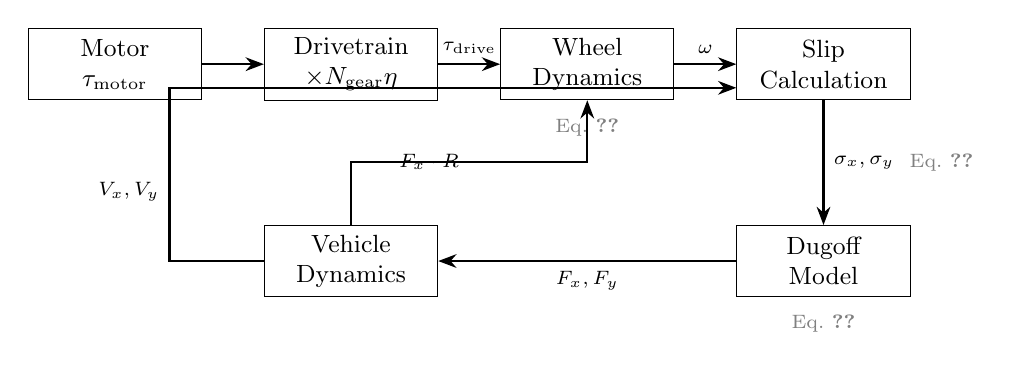
\begin{tikzpicture}[
    block/.style={rectangle, draw, minimum width=2.2cm, minimum height=0.9cm, align=center, font=\small},
    sum/.style={circle, draw, minimum size=0.4cm},
    arrow/.style={-{Stealth[scale=1.0]}, thick}
]

% Blocks - Top row
\node[block] (motor) at (0, 0) {Motor\\$\tau_{\text{motor}}$};
\node[block] (drivetrain) at (3, 0) {Drivetrain\\$\times N_{\text{gear}} \eta$};
\node[block] (wheel) at (6, 0) {Wheel\\Dynamics};
\node[block] (slip) at (9, 0) {Slip\\Calculation};

% Blocks - Bottom row
\node[block] (dugoff) at (9, -2.5) {Dugoff\\Model};
\node[block] (vehicle) at (3, -2.5) {Vehicle\\Dynamics};

% Arrows - Top row
\draw[arrow] (motor) -- (drivetrain);
\draw[arrow] (drivetrain) -- (wheel) node[midway, above, font=\scriptsize] {$\tau_{\text{drive}}$};
\draw[arrow] (wheel) -- (slip) node[midway, above, font=\scriptsize] {$\omega$};

% Arrows - Right side
\draw[arrow] (slip) -- (dugoff) node[midway, right, font=\scriptsize] {$\sigma_x, \sigma_y$};

% Arrows - Bottom
\draw[arrow] (dugoff) -- (vehicle) node[midway, below, font=\scriptsize] {$F_x, F_y$};

% Feedback arrows
\draw[arrow] (vehicle.north) -- ++(0, 0.8) -| (wheel.south) node[pos=0.25, left, font=\scriptsize] {$F_x \cdot R$};
\draw[arrow] (vehicle.west) -- ++(-1.2, 0) |- ($(slip.west) + (0, -0.3)$) node[pos=0.2, left, font=\scriptsize] {$V_x, V_y$};

% Equation labels
\node[font=\scriptsize, gray] at (6, -0.8) {Eq.~\ref{eq:wheel_dynamics}};
\node[font=\scriptsize, gray] at (10.5, -1.25) {Eq.~\ref{eq:slip_ratio}};
\node[font=\scriptsize, gray] at (9, -3.3) {Eq.~\ref{eq:Fx_dugoff}};

\end{tikzpicture}
\caption{Closed-loop system architecture for hybrid torque-slip model}
\label{fig:closed_loop}
\end{figure}

\subsection{Causality Chain}

At each timestep $k$:

\begin{enumerate}
    \item \textbf{Input:} Motor torque command $\tau_{\text{motor}}$
    \item \textbf{Drivetrain:} $\tau_{\text{wheel}} = \tau_{\text{motor}} \cdot N_{\text{gear}} \cdot \eta$
    \item \textbf{Wheel dynamics:} Integrate $\omega[k+1]$ using Eq.~\ref{eq:wheel_integration}
    \item \textbf{Slip calculation:} Compute $\sigma_x, \sigma_y$ using Eq.~\ref{eq:slip_ratio}
    \item \textbf{Dugoff model:} Compute $F_x, F_y$ using Eq.~\ref{eq:Fx_dugoff}, \ref{eq:Fy_dugoff}
    \item \textbf{Vehicle dynamics:} Update $V_x, V_y$ from tire forces
    \item \textbf{Feedback:} Tire reaction torque $F_x \cdot R$ affects next wheel integration
\end{enumerate}

\subsection{Key Insight: Feedback Loop}

The tire force $F_x$ appears on \textbf{both sides} of the system:
\begin{itemize}
    \item \textbf{Output:} Accelerates the vehicle ($m\dot{V}_x = \sum F_x$)
    \item \textbf{Feedback:} Decelerates the wheel ($I_w \dot{\omega} = \tau - F_x R$)
\end{itemize}

This creates natural self-regulation:
\begin{itemize}
    \item High slip $\rightarrow$ reduced $F_x$ (saturation) $\rightarrow$ wheel accelerates less
    \item Low slip $\rightarrow$ high $F_x$ $\rightarrow$ wheel slows toward free-rolling
\end{itemize}

%=============================================================================
\section{Lateral Velocity and Slip Angle Computation}
%=============================================================================

\subsection{Front Axle Lateral Velocity}

Lateral velocity at front tire contact patch:
\begin{equation}
V_{y,\text{front}} = V_y + \dot{\psi} \cdot L_f - V_x \tan(\delta)
\end{equation}

where:
\begin{itemize}
    \item $V_y$ -- vehicle lateral velocity at CoG (m/s)
    \item $\dot{\psi}$ -- yaw rate (rad/s)
    \item $\delta$ -- steering angle (rad)
\end{itemize}

\subsection{Rear Axle Lateral Velocity}

\begin{equation}
V_{y,\text{rear}} = V_y - \dot{\psi} \cdot L_r
\end{equation}

\subsection{Per-Wheel Lateral Slip Ratio}

For front wheels (with Ackermann steering):
\begin{align}
\sigma_{y,\text{fl}} &= \frac{V_y + \dot{\psi} L_f - V_x \tan(\delta_{\text{FL}})}{V_x} \\
\sigma_{y,\text{fr}} &= \frac{V_y + \dot{\psi} L_f - V_x \tan(\delta_{\text{FR}})}{V_x}
\end{align}

For rear wheels:
\begin{align}
\sigma_{y,\text{rl}} = \sigma_{y,\text{rr}} &= \frac{V_y - \dot{\psi} L_r}{V_x}
\end{align}

%=============================================================================
\section{Torque-Only vs Hybrid Model}
\label{sec:comparison}
%=============================================================================

\subsection{Torque-Only Model (Current Default)}

Direct force computation without wheel dynamics:
\begin{equation}
F_x = \min\left( \frac{\tau_{\text{motor}} \cdot N_{\text{gear}} \cdot \eta}{R}, \mu F_z \right)
\end{equation}

\textbf{Advantages:}
\begin{itemize}
    \item Simple, fast computation
    \item No additional state variables
    \item Stable at all speeds
    \item Captures traction limiting
\end{itemize}

\textbf{Limitations:}
\begin{itemize}
    \item Cannot model wheel spin ($\omega \gg V_x/R$)
    \item Cannot model wheel lock ($\omega = 0$ while $V_x > 0$)
    \item Slip ratio is estimated, not computed
    \item No TCS/ABS testing capability
\end{itemize}

\subsection{Hybrid Model}

Full causality: $\tau_{\text{motor}} \rightarrow \omega \rightarrow \sigma_x \rightarrow F_x$

\textbf{Advantages:}
\begin{itemize}
    \item Physical wheel spin and lock behavior
    \item Natural slip development
    \item Full Dugoff slip-force curve (including peak and sliding)
    \item TCS/ABS algorithm testing
    \item Realistic launch and braking dynamics
\end{itemize}

\textbf{Limitations:}
\begin{itemize}
    \item Additional state variables (4 wheel speeds)
    \item Requires smaller timestep for stability
    \item More complex initialization
\end{itemize}

\subsection{Model Selection Guide}

\begin{table}[H]
\centering
\begin{tabular}{lcc}
\toprule
\textbf{Use Case} & \textbf{Torque-Only} & \textbf{Hybrid} \\
\midrule
Path following & $\checkmark$ & $\checkmark$ \\
Energy estimation & $\checkmark$ & $\checkmark$ \\
Traction limiting & $\checkmark$ & $\checkmark$ \\
Wheel spin detection & & $\checkmark$ \\
ABS/TCS development & & $\checkmark$ \\
Stability control & & $\checkmark$ \\
Loss of control & & $\checkmark$ \\
\bottomrule
\end{tabular}
\caption{Model selection based on use case}
\end{table}

%=============================================================================
\section{Implementation Algorithm}
%=============================================================================

\subsection{Torque-Only Algorithm}

\textbf{Step 1: Compute Normal Loads}
\begin{enumerate}
    \item Static distribution from geometry
    \item Load transfer: $\Delta F_z = m a_x h_{\text{cg}} / L$
    \item Per-wheel loads
\end{enumerate}

\textbf{Step 2: Compute Demanded Force}
\begin{equation}
F_{x,\text{demanded}} = \frac{\tau_{\text{motor}} \cdot N_{\text{gear}} \cdot \eta}{R}
\end{equation}

\textbf{Step 3: Apply Friction Limit}
\begin{equation}
F_x = \min(|F_{x,\text{demanded}}|, \mu F_z) \cdot \text{sgn}(F_{x,\text{demanded}})
\end{equation}

\textbf{Step 4: Update Vehicle Dynamics}
\begin{equation}
a = \frac{\sum F_x - F_{\text{drag}} - F_{\text{roll}}}{m}
\end{equation}

\subsection{Hybrid Algorithm}

\textbf{Step 1: Compute Normal Loads} (same as torque-only)

\textbf{Step 2: Compute Slip Ratios from Current Wheel Speeds}
\begin{equation}
\sigma_x = \frac{\omega R - V_x}{\max(|V_x|, |\omega R|, V_{\min})}
\end{equation}

\textbf{Step 3: Compute Tire Forces (Dugoff)}
\begin{align}
\lambda &= \frac{\mu F_z}{2\sqrt{(C_x \sigma_x)^2 + (C_y \sigma_y)^2}} \\
f(\lambda) &= \begin{cases} (2-\lambda)\lambda & \lambda < 1 \\ 1 & \lambda \geq 1 \end{cases} \\
F_x &= C_x \sigma_x f(\lambda)
\end{align}

\textbf{Step 4: Update Wheel Dynamics}
\begin{equation}
\omega[k+1] = \omega[k] + \frac{\Delta t}{I_w}(\tau_{\text{drive}} - \tau_{\text{brake}} \cdot \text{sgn}(\omega) - F_x R)
\end{equation}

\textbf{Step 5: Update Vehicle Dynamics}
\begin{equation}
V_x[k+1] = V_x[k] + \frac{\Delta t}{m}(\sum F_x - F_{\text{drag}} - F_{\text{roll}})
\end{equation}

\subsection{Complete Discrete-Time State Update}

\begin{align}
\omega_i[k+1] &= \omega_i[k] + \Delta t \cdot \dot{\omega}_i \quad \text{(for each wheel $i$)} \\
V_x[k+1] &= V_x[k] + \Delta t \cdot a_x \\
\dot{\psi}[k] &= \frac{V_x[k]}{L} \tan(\delta[k]) \quad \text{(or from lateral dynamics)} \\
\psi[k+1] &= \psi[k] + \Delta t \cdot \dot{\psi}[k] \\
x[k+1] &= x[k] + \Delta t \cdot V_x[k] \cos(\psi[k]) \\
y[k+1] &= y[k] + \Delta t \cdot V_x[k] \sin(\psi[k])
\end{align}

%=============================================================================
\section{Surface Friction Coefficients}
%=============================================================================

\subsection{Mining Haul Road Conditions}

\begin{table}[H]
\centering
\begin{tabular}{lcc}
\toprule
\textbf{Surface} & $\mu_{\text{peak}}$ & $\mu_{\text{slide}}$ \\
\midrule
Dry pavement & 0.85 & 0.70 \\
Compact gravel & 0.72 & 0.60 \\
Loose gravel & 0.55 & 0.45 \\
Iron ore dust (dry) & 0.45 & 0.35 \\
Iron ore dust (wet) & 0.30 & 0.22 \\
Mud & 0.25 & 0.18 \\
Sand (loose) & 0.40 & 0.32 \\
\bottomrule
\end{tabular}
\caption{Friction coefficients for Pilbara mining conditions}
\end{table}

\subsection{Effect of Surface Friction}

The surface friction $\mu$ directly affects:

\begin{enumerate}
    \item \textbf{Maximum traction force:} $F_{x,\max} = \mu F_z$
    \item \textbf{Maximum acceleration:} $a_{\max} = \mu g$ (flat road)
    \item \textbf{Stopping distance:} $d_{\text{stop}} = \frac{v_0^2}{2\mu g}$
    \item \textbf{Friction utilization:} Lower $\mu$ means earlier saturation ($\lambda < 1$)
\end{enumerate}

%=============================================================================
\section{Implementation Parameters}
%=============================================================================

\subsection{Heavy-Duty Electric Vehicle Mining Truck}

\begin{table}[H]
\centering
\begin{tabular}{lll}
\toprule
\textbf{Parameter} & \textbf{Value} & \textbf{Unit} \\
\midrule
Mass (empty) & 218,000 & kg \\
Mass (loaded) & 538,000 & kg \\
Wheelbase $L$ & 6.3 & m \\
Track width $W$ & 4.0 & m \\
CG height $h_{\text{cg}}$ & 2.8 & m \\
Tire radius $R$ & 1.93 & m \\
Gear ratio $N_{\text{gear}}$ & 9.0 & - \\
Drivetrain efficiency $\eta$ & 0.92 & - \\
Motor max torque & 145,000 & N$\cdot$m \\
Motor max power & 2,100 & kW \\
\bottomrule
\end{tabular}
\caption{Vehicle parameters}
\end{table}

\begin{table}[H]
\centering
\begin{tabular}{lll}
\toprule
\textbf{Parameter} & \textbf{Value} & \textbf{Unit} \\
\midrule
$C_{x,\text{base}}$ & 280,000 & N \\
$C_{y,\text{base}}$ & 220,000 & N \\
$F_{z,\text{ref}}$ & 100,000 & N \\
$I_w$ (front) & 800 & kg$\cdot$m$^2$ \\
$I_w$ (rear) & 1,200 & kg$\cdot$m$^2$ \\
\bottomrule
\end{tabular}
\caption{Tire and wheel parameters}
\end{table}

\begin{table}[H]
\centering
\begin{tabular}{lll}
\toprule
\textbf{Parameter} & \textbf{Value} & \textbf{Unit} \\
\midrule
Maximum steering angle $\delta_{\max}$ & 35 & deg \\
Steering rate limit $\dot{\delta}_{\max}$ & 45 & deg/s \\
Ackermann percentage $\alpha_{\text{ack}}$ & 100 & \% \\
Speed limit start $v_{\text{start}}$ & 8 & m/s \\
Speed limit end $v_{\text{end}}$ & 25 & m/s \\
High-speed ratio $r_{\text{high}}$ & 0.35 & - \\
Brake bias (front) $\beta_{\text{front}}$ & 0.40 & - \\
\bottomrule
\end{tabular}
\caption{Steering and brake parameters}
\end{table}

%=============================================================================
\section{Validation and Benchmarks}
%=============================================================================

\subsection{Expected Behavior}

\textbf{Scenario 1: Acceleration on gravel ($\mu = 0.72$)}

Heavy-Duty Electric Vehicle empty (218 tons):
\begin{align}
F_{z,\text{rear}} &\approx 0.60 \times 218{,}000 \times 9.81 = 1{,}283{,}000 \text{ N} \\
F_{x,\text{max}} &= 0.72 \times 1{,}283{,}000 = 924{,}000 \text{ N} \\
a_{\max} &= \frac{924{,}000}{218{,}000} = 4.2 \text{ m/s}^2
\end{align}

\textbf{Scenario 2: Acceleration on wet dust ($\mu = 0.30$)}

\begin{align}
F_{x,\text{max}} &= 0.30 \times 1{,}283{,}000 = 385{,}000 \text{ N} \\
a_{\max} &= \frac{385{,}000}{218{,}000} = 1.8 \text{ m/s}^2
\end{align}

\textbf{Result:} Acceleration limited to 1.8 m/s$^2$ on wet dust vs 4.2 m/s$^2$ on gravel.

\subsection{Stopping Distance Comparison}

For $v_0 = 50$ km/h = 13.9 m/s:

\begin{align}
d_{\text{gravel}} &= \frac{13.9^2}{2 \times 0.72 \times 9.81} = 13.7 \text{ m} \\
d_{\text{wet dust}} &= \frac{13.9^2}{2 \times 0.30 \times 9.81} = 32.8 \text{ m}
\end{align}

Stopping distance increases 2.4$\times$ on wet dust compared to gravel.

\subsection{Minimum Turn Radius Verification}

At $\delta_{\max} = 35°$ with $L = 6.3$ m:
\begin{equation}
R_{\min} = \frac{6.3}{\tan(35°)} = 9.0 \text{ m}
\end{equation}

Inner wheel turn radius: $R_{\text{inner}} = 9.0 - 2.0 = 7.0$ m

This matches the expected tight-turn capability for pit operations.

%=============================================================================
\section{Future Enhancements}
%=============================================================================

\subsection{Short-Term (V2.5)}
\begin{itemize}
    \item[$\checkmark$] Wheel rotational dynamics (this document)
    \item[$\checkmark$] Hybrid torque-slip model
    \item[$\checkmark$] Ackermann steering geometry
    \item Combined longitudinal-lateral friction circle
\end{itemize}

\subsection{Medium-Term (V3)}
\begin{itemize}
    \item 3-DOF vehicle dynamics (add $V_y$, $\dot{\psi}$ as states)
    \item Oversteer/understeer simulation
    \item Loss of control scenarios
    \item Steering aligning torque feedback
\end{itemize}

\subsection{Long-Term (V4)}
\begin{itemize}
    \item 6-DOF dynamics (roll, pitch, heave)
    \item Suspension dynamics
    \item Rollover detection and prevention
    \item Four-wheel steering option
\end{itemize}

%=============================================================================
\section{Conclusion}
%=============================================================================

This document presents a comprehensive vehicle dynamics model with:

\textbf{Steering System:}
\begin{itemize}
    \item Ackermann geometry for individual wheel angles
    \item Configurable Ackermann percentage
    \item Speed-dependent steering limit
    \item Rate limiting for hydraulic systems
\end{itemize}

\textbf{Tire Modeling:}
\begin{itemize}
    \item Torque-only model for simple traction limiting
    \item Hybrid torque-slip model with wheel dynamics
    \item Full Dugoff slip-force characteristic
    \item Friction circle constraint
\end{itemize}

\textbf{Vehicle Dynamics:}
\begin{itemize}
    \item Load transfer during acceleration/braking
    \item Per-wheel normal load computation
    \item Force-based longitudinal dynamics
    \item Surface friction effects
\end{itemize}

This forms a solid foundation for autonomous mining vehicle simulation and control algorithm development.

%=============================================================================
\begin{thebibliography}{9}

\bibitem{dugoff1970}
Dugoff, H., Fancher, P. S., and Segel, L. (1970).
\textit{An Analysis of Tire Traction Properties and Their Influence on Vehicle Dynamic Performance}.
SAE Technical Paper 700377.

\bibitem{rajamani2012}
Rajamani, R. (2012). \textit{Vehicle Dynamics and Control}. Springer.

\bibitem{gillespie1992}
Gillespie, T. D. (1992). \textit{Fundamentals of Vehicle Dynamics}. SAE International.

\bibitem{pacejka2012}
Pacejka, H. (2012). \textit{Tire and Vehicle Dynamics}, 3rd Edition. Butterworth-Heinemann.

\bibitem{iso8855}
ISO 8855:2011. Road vehicles -- Vehicle dynamics and road-holding ability -- Vocabulary.

\end{thebibliography}

\appendix



\section{Sensor Models}

\subsection{Sensor Noise Models}

\subsubsection{Gaussian White Noise}

Additive zero-mean Gaussian noise:
\begin{equation}
y = x_{\text{truth}} + \mathcal{N}(0, \sigma^2)
\end{equation}

where $\mathcal{N}(0, \sigma^2)$ is normal distribution with standard deviation $\sigma$.

\textbf{Implementation:} Box-Muller transform:
\begin{align}
U_1, U_2 &\sim \mathcal{U}(0, 1) \quad \text{(uniform random)} \\
Z_1 &= \sqrt{-2 \ln U_1} \cos(2\pi U_2) \\
Z_2 &= \sqrt{-2 \ln U_1} \sin(2\pi U_2)
\end{align}

where $Z_1, Z_2 \sim \mathcal{N}(0, 1)$.

Scaled noise: $\sigma Z_1 \sim \mathcal{N}(0, \sigma^2)$.

\subsubsection{Random Walk}

Brownian motion (Wiener process):
\begin{equation}
dx = \sigma_{\text{rw}} dW
\end{equation}

where $dW \sim \mathcal{N}(0, dt)$ is Wiener increment.

Discrete implementation:
\begin{equation}
x_{k+1} = x_k + \sigma_{\text{rw}} \sqrt{\Delta t} \cdot \mathcal{N}(0, 1)
\end{equation}

\textbf{Example:} GNSS position drift with $\sigma_{\text{rw}} = 0.1$ m/$\sqrt{\text{s}}$.

\subsubsection{Gauss-Markov Process}

First-order Markov process (exponentially correlated noise):
\begin{equation}
\frac{db}{dt} = -\frac{1}{\tau} b + w(t)
\end{equation}

where:
\begin{itemize}
    \item $b$ -- bias state
    \item $\tau$ -- correlation time constant (s)
    \item $w(t) \sim \mathcal{N}(0, \sigma_w^2)$ -- white noise driving term
\end{itemize}

\textbf{Discrete solution:}
\begin{equation}
b_{k+1} = e^{-\Delta t / \tau} b_k + \sigma_b \sqrt{1 - e^{-2\Delta t / \tau}} \cdot \mathcal{N}(0, 1)
\end{equation}

where $\sigma_b$ is steady-state bias standard deviation.

\textbf{Steady-state variance:}
\begin{equation}
\sigma_b^2 = \frac{\tau \sigma_w^2}{2}
\end{equation}

\subsection{IMU Sensor Model}

\subsubsection{Gyroscope Model}

Measured angular velocity:
\begin{equation}
\omega_{\text{meas}} = \omega_{\text{truth}} + b_{\text{gyro}} + n_{\text{gyro}}
\end{equation}

where:
\begin{itemize}
    \item $\omega_{\text{truth}}$ -- true angular velocity (rad/s)
    \item $b_{\text{gyro}}$ -- time-varying bias (Gauss-Markov, $\tau = 1800$ s)
    \item $n_{\text{gyro}} \sim \mathcal{N}(0, \sigma_{\text{gyro}}^2)$ -- white noise ($\sigma = 0.1°$/s)
\end{itemize}

\textbf{Bias evolution:}
\begin{equation}
b_{\text{gyro},k+1} = \beta b_{\text{gyro},k} + \sigma_b \sqrt{1 - \beta^2} \cdot \mathcal{N}(0, 1)
\end{equation}

where $\beta = \exp(-\Delta t / \tau)$.

\subsubsection{Accelerometer Model}

Measured acceleration (body frame):
\begin{equation}
\mathbf{a}_{\text{meas}} = \mathbf{a}_{\text{truth}} + \mathbf{b}_{\text{accel}} + \mathbf{n}_{\text{accel}}
\end{equation}

\textbf{Truth values in body frame:}
\begin{align}
a_{x,\text{truth}} &= \frac{dv}{dt} \quad \text{(longitudinal acceleration)} \\
a_{y,\text{truth}} &= v \cdot \dot{\psi} \quad \text{(centripetal acceleration)} \\
a_{z,\text{truth}} &= -g = -9.81 \text{ m/s}^2 \quad \text{(gravity, body Z up)}
\end{align}

\textbf{Bias:} Gauss-Markov with $\tau = 3600$ s (1 hour), $\sigma_b = 0.02$ m/s$^2$.

\textbf{White noise:} $\sigma_{\text{accel}} = 0.05$ m/s$^2$.

\subsubsection{Gravity Compensation}

Accelerometers measure \textbf{specific force} (excluding gravity). For a stationary vehicle:
\begin{equation}
\mathbf{a}_{\text{meas}} = -\mathbf{g}_{\text{body}} + \text{bias} + \text{noise}
\end{equation}

where $\mathbf{g}_{\text{body}} = [0, 0, -9.81]^\top$ m/s$^2$ in body frame (Z-up).

During motion:
\begin{equation}
\mathbf{a}_{\text{meas}} = \mathbf{a}_{\text{vehicle}} - \mathbf{g}_{\text{body}} + \text{bias} + \text{noise}
\end{equation}

\subsection{GNSS Sensor Model}

\subsubsection{Position Measurement}

Latitude and longitude with random walk drift:
\begin{align}
\phi_{\text{meas}} &= \phi_{\text{truth}} + d_{\phi} + \mathcal{N}(0, \sigma_{\phi}^2) \\
\lambda_{\text{meas}} &= \lambda_{\text{truth}} + d_{\lambda} + \mathcal{N}(0, \sigma_{\lambda}^2)
\end{align}

where:
\begin{itemize}
    \item $d_{\phi}, d_{\lambda}$ -- random walk drift ($\sigma_{\text{rw}} = 0.1$ m/$\sqrt{\text{s}}$)
    \item $\sigma_{\phi} = 2.0$ m / $m_{\phi}$ -- white noise (latitude)
    \item $\sigma_{\lambda} = 2.0$ m / $m_{\lambda}$ -- white noise (longitude)
\end{itemize}

\subsubsection{Velocity Measurement (NED Frame)}

North-East velocity:
\begin{align}
v_{N,\text{meas}} &= v_N + \mathcal{N}(0, 0.1^2) \\
v_{E,\text{meas}} &= v_E + \mathcal{N}(0, 0.1^2)
\end{align}

where $v_N = v \sin(\psi)$ and $v_E = v \cos(\psi)$ from body velocity transformation.

\subsubsection{Circular Error Probable (CEP)}

The 50\% probability error circle radius:
\begin{equation}
\text{CEP} = 0.59(\sigma_N + \sigma_E) \approx 1.2 \text{ m}
\end{equation}

for $\sigma_N = \sigma_E = 2.0$ m.

\section{Wheel Speed Encoder Model}

\subsubsection{Quantization Model}

Encoder with $N_{\text{ticks}}$ pulses per revolution:
\begin{equation}
\text{Resolution} = \frac{2\pi}{N_{\text{ticks}}} \text{ rad}
\end{equation}

Quantized measurement:
\begin{equation}
\omega_{\text{quant}} = \left\lfloor \frac{\omega_{\text{truth}}}{\text{Resolution}} \right\rceil \cdot \text{Resolution}
\end{equation}

where $\lfloor \cdot \rceil$ denotes rounding to nearest integer.

\subsubsection{Total Encoder Noise}

Combined quantization and sensor noise:
\begin{equation}
\omega_{\text{meas}} = \omega_{\text{quant}} + \mathcal{N}(0, \sigma_{\omega}^2)
\end{equation}

where $\sigma_{\omega} = 0.5$ rad/s (white noise).

\subsubsection{Per-Wheel Variation}

Simulate tire pressure and slip variations:
\begin{equation}
\omega_i = \omega_{\text{meas}} \cdot (1 + u_i)
\end{equation}

where $u_i \sim \mathcal{U}(-0.02, +0.02)$ is uniform random variable (2\% variation).

\subsection{Radar Sensor Model}

\subsubsection{Range Measurement}

Simulated stationary target at fixed distance:
\begin{equation}
r_{\text{meas}} = r_{\text{truth}} + \mathcal{N}(0, \sigma_r^2)
\end{equation}

where $r_{\text{truth}} = 50.0$ m and $\sigma_r = 0.2$ m.

\subsubsection{Doppler Velocity}

Relative radial velocity (closing speed):
\begin{equation}
v_{\text{rel}} = v_{\text{ego}} \cos(\theta)
\end{equation}

where $\theta$ is angle between vehicle heading and line-of-sight to target.

For target dead ahead ($\theta = 0$):
\begin{equation}
v_{\text{meas}} = v_{\text{truth}} + \mathcal{N}(0, \sigma_v^2)
\end{equation}

where $\sigma_v = 0.1$ m/s.

\subsubsection{Angle Measurement}

Azimuth angle to target:
\begin{equation}
\alpha_{\text{meas}} = \alpha_{\text{truth}} + \mathcal{N}(0, \sigma_{\alpha}^2)
\end{equation}

where $\alpha_{\text{truth}} = 0°$ (dead ahead) and $\sigma_{\alpha} = 0.5°$.

% -------------------- Appendices from Sensor/Kinematics document --------------------

\section{Coordinate Systems and Transformations}

\subsection{Reference Frames}

\subsubsection{Global Inertial Frame (World)}

Fixed reference frame with origin at simulation start:
\begin{itemize}
    \item $X$ -- East (or initial vehicle forward direction)
    \item $Y$ -- North (or initial vehicle left direction)
    \item $Z$ -- Up (vertical, right-hand rule)
\end{itemize}

Vehicle state in global frame: $(x, y, \psi)$ where $\psi$ is heading angle (yaw) measured counterclockwise from $X$-axis.

\subsubsection{Vehicle Body Frame}

Moving frame attached to vehicle with origin at rear axle center:
\begin{itemize}
    \item $x_b$ -- Forward (longitudinal)
    \item $y_b$ -- Left (lateral)
    \item $z_b$ -- Up (vertical)
\end{itemize}

Vehicle velocity in body frame: $v$ (longitudinal speed, m/s).

\subsubsection{North-East-Down (NED) Frame}

Navigation frame used by GNSS:
\begin{itemize}
    \item $N$ -- North
    \item $E$ -- East
    \item $D$ -- Down (toward Earth center)
\end{itemize}

\subsection{Coordinate Transformations}

\subsubsection{Body to Global}

Position rate of change:
\begin{align}
\dot{x} &= v \cos(\psi) \label{eq:xdot}\\
\dot{y} &= v \sin(\psi) \label{eq:ydot}
\end{align}

Rotation matrix from body to global:
\begin{equation}
\mathbf{R}_b^g = \begin{bmatrix}
\cos\psi & -\sin\psi & 0 \\
\sin\psi & \cos\psi & 0 \\
0 & 0 & 1
\end{bmatrix}
\end{equation}

\subsubsection{Body to NED}

Velocity transformation:
\begin{align}
v_N &= v \sin(\psi) \\
v_E &= v \cos(\psi) \\
v_D &= 0 \quad \text{(ground vehicle)}
\end{align}

\subsubsection{Local XY to WGS84}

Flat Earth approximation for short distances ($<10$ km):
\begin{align}
\text{meters per degree latitude:} \quad m_{\phi} &= 111{,}320 \text{ m} \\
\text{meters per degree longitude:} \quad m_{\lambda} &= 111{,}320 \cdot \cos(\phi_0) \text{ m}
\end{align}

Position conversion:
\begin{align}
\phi &= \phi_0 + \frac{y}{m_{\phi}} \\
\lambda &= \lambda_0 + \frac{x}{m_{\lambda}}
\end{align}

where $(\phi_0, \lambda_0)$ is the origin in WGS84 coordinates (latitude, longitude in degrees).

\section{Bicycle Model Kinematics}

\subsection{Model Assumptions}

\begin{enumerate}
    \item \textbf{No slip:} Pure rolling condition (wheels do not slide)
    \item \textbf{Planar motion:} Vehicle remains on flat ground (no pitch/roll)
    \item \textbf{Point mass:} Neglect rotational inertia about vertical axis
    \item \textbf{Rear-axle reference:} Kinematic center at rear axle midpoint
\end{enumerate}

\subsection{Kinematic Equations}

The bicycle model reduces a four-wheeled vehicle to two wheels separated by wheelbase $L$:

\begin{equation}
\begin{aligned}
\dot{x} &= v \cos(\psi) \\
\dot{y} &= v \sin(\psi) \\
\dot{\psi} &= \frac{v}{L} \tan(\delta)
\end{aligned}
\label{eq:bicycle_model}
\end{equation}

where:
\begin{itemize}
    \item $(x, y)$ -- position of rear axle center in global frame (m)
    \item $\psi$ -- heading angle (rad)
    \item $v$ -- longitudinal velocity (m/s)
    \item $\delta$ -- virtual bicycle steering angle (rad)
    \item $L$ -- wheelbase (m)
\end{itemize}

\subsection{Derivation of Yaw Rate}

\textbf{Step 1:} Front wheel velocity perpendicular to wheel heading (no-slip):
\begin{equation}
v_f = \frac{v}{\cos(\delta)}
\end{equation}

\textbf{Step 2:} Lateral component of front wheel velocity:
\begin{equation}
v_{f,\text{lateral}} = v_f \sin(\delta) = v \tan(\delta)
\end{equation}

\textbf{Step 3:} Angular velocity about rear axle (instantaneous center of rotation):
\begin{equation}
\dot{\psi} = \frac{v_{f,\text{lateral}}}{L} = \frac{v \tan(\delta)}{L}
\end{equation}

\subsection{Turning Radius}

From the yaw rate equation:
\begin{equation}
R = \frac{L}{\tan(\delta)}
\end{equation}

For small angles ($|\delta| < 0.2$ rad $\approx 11°$):
\begin{equation}
\tan(\delta) \approx \delta \implies R \approx \frac{L}{\delta}
\end{equation}

\subsection{Discrete-Time Integration}

Using Euler forward integration with timestep $\Delta t$:

\begin{align}
\psi_{k+1} &= \psi_k + \Delta t \cdot \frac{v_k}{L} \tan(\delta_k) \\
x_{k+1} &= x_k + \Delta t \cdot v_k \cos(\psi_k) \\
y_{k+1} &= y_k + \Delta t \cdot v_k \sin(\psi_k)
\end{align}

\textbf{Stability condition:} To prevent integration instability:
\begin{equation}
\Delta t < \frac{L}{v_{\max} \tan(\delta_{\max})}
\end{equation}

For $L=2.8$ m, $v_{\max}=60$ m/s, $\delta_{\max}=35° \approx 0.61$ rad:
\begin{equation}
\Delta t < 0.067 \text{ s} = 67 \text{ ms}
\end{equation}

Chosen timestep: $\Delta t = 10$ ms provides 6.7$\times$ safety margin.

\section{Ackermann Steering Geometry}

\subsection{Problem Statement}

Real vehicles have two front wheels that must turn at different angles to maintain pure rolling (no tire scrubbing). All wheels must rotate about a common \textbf{instantaneous center of rotation (ICR)}.

\subsection{Geometric Configuration}

\begin{center}
\begin{tabular}{ll}
\toprule
Parameter & Symbol \\
\midrule
Wheelbase & $L$ \\
Track width (front) & $W$ \\
Virtual steering angle & $\delta$ \\
Turning radius (rear axle to ICR) & $R$ \\
\bottomrule
\end{tabular}
\end{center}

\subsection{Derivation}

\textbf{Step 1:} Turning radius from bicycle model:
\begin{equation}
R = \frac{L}{\tan(\delta)}
\end{equation}

\textbf{Step 2:} Inner and outer wheel radii:
\begin{align}
R_{\text{inner}} &= R - \frac{W}{2} \\
R_{\text{outer}} &= R + \frac{W}{2}
\end{align}

\textbf{Step 3:} Front wheel angles from geometry:
\begin{align}
\delta_{\text{inner}} &= \arctan\left(\frac{L}{R_{\text{inner}}}\right) = \arctan\left(\frac{L}{R - W/2}\right) \\
\delta_{\text{outer}} &= \arctan\left(\frac{L}{R_{\text{outer}}}\right) = \arctan\left(\frac{L}{R + W/2}\right)
\end{align}

\subsection{Turn Direction Convention}

For \textbf{left turn} ($\delta > 0$):
\begin{align}
\delta_{FL} &= \arctan\left(\frac{L}{R - W/2}\right) \quad \text{(inner, larger angle)} \\
\delta_{FR} &= \arctan\left(\frac{L}{R + W/2}\right) \quad \text{(outer, smaller angle)}
\end{align}

For \textbf{right turn} ($\delta < 0$):
\begin{align}
\delta_{FR} &= \arctan\left(\frac{L}{R - W/2}\right) \quad \text{(inner, larger magnitude)} \\
\delta_{FL} &= \arctan\left(\frac{L}{R + W/2}\right) \quad \text{(outer, smaller magnitude)}
\end{align}

\subsection{Small Angle Approximation}

For $|\delta| \ll 1$:
\begin{align}
\delta_{\text{inner}} &\approx \frac{L}{R - W/2} = \delta \left(1 + \frac{W}{2R}\right) \\
\delta_{\text{outer}} &\approx \frac{L}{R + W/2} = \delta \left(1 - \frac{W}{2R}\right)
\end{align}

\section{Longitudinal Dynamics}

\subsection{Force Balance}

Newton's second law in longitudinal direction:
\begin{equation}
m \frac{dv}{dt} = F_{\text{motor}} - F_{\text{brake}} - F_{\text{drag}} - F_{\text{roll}}
\end{equation}

where $m$ is vehicle mass (kg) and $v$ is longitudinal velocity (m/s).

\subsection{Motor Force}

Electric motor torque converted to wheel force:
\begin{equation}
F_{\text{motor}} = \frac{T_{\text{motor}} \cdot N_{\text{gear}} \cdot \eta_{\text{drivetrain}}}{r_{\text{wheel}}}
\end{equation}

where:
\begin{itemize}
    \item $T_{\text{motor}}$ -- motor shaft torque (Nm)
    \item $N_{\text{gear}}$ -- gear ratio (dimensionless)
    \item $\eta_{\text{drivetrain}}$ -- drivetrain efficiency (typically 0.92)
    \item $r_{\text{wheel}}$ -- effective wheel radius (m)
\end{itemize}

\subsection{Power Constraint}

Motors are torque-limited at low speed and power-limited at high speed:
\begin{equation}
P_{\text{motor}} = T_{\text{motor}} \cdot \omega_{\text{motor}}
\end{equation}

Motor angular velocity:
\begin{equation}
\omega_{\text{motor}} = \frac{v}{r_{\text{wheel}}} \cdot N_{\text{gear}}
\end{equation}

Maximum torque at given speed:
\begin{equation}
T_{\text{motor}}^{\max}(v) = \frac{P_{\text{motor}}^{\max}}{\omega_{\text{motor}}(v)} = \frac{P_{\text{motor}}^{\max} \cdot r_{\text{wheel}}}{v \cdot N_{\text{gear}}}
\end{equation}

\subsection{Aerodynamic Drag}

Quadratic drag force:
\begin{equation}
F_{\text{drag}} = \frac{1}{2} \rho C_d A v^2 = C_{\text{drag}} v |v|
\end{equation}

where:
\begin{itemize}
    \item $\rho$ -- air density (\SI{1.225}{kg/m^3} at sea level)
    \item $C_d$ -- drag coefficient (dimensionless, 0.25--1.2 depending on vehicle)
    \item $A$ -- frontal area (m$^2$)
    \item $C_{\text{drag}} = \frac{1}{2}\rho C_d A$ -- combined drag constant
\end{itemize}

\subsection{Rolling Resistance}

Simplified constant friction model:
\begin{equation}
F_{\text{roll}} = C_{\text{roll}} \cdot \text{sign}(v)
\end{equation}

where $C_{\text{roll}}$ is rolling resistance force magnitude (N).

More detailed model:
\begin{equation}
F_{\text{roll}} = \mu_{\text{roll}} \cdot m \cdot g
\end{equation}

where $\mu_{\text{roll}}$ is rolling resistance coefficient (0.01--0.03 for asphalt).

\subsection{Friction Braking}

Brake force proportional to pedal input:
\begin{equation}
F_{\text{brake}} = \frac{p_{\text{brake}}}{100} \cdot \frac{T_{\text{brake}}^{\max}}{r_{\text{wheel}}}
\end{equation}

where $p_{\text{brake}} \in [0, 100]$ is brake pedal percentage.

\subsection{Velocity Update}

Acceleration:
\begin{equation}
a = \frac{F_{\text{motor}} - F_{\text{brake}} - F_{\text{drag}} - F_{\text{roll}}}{m}
\end{equation}

Discrete velocity update:
\begin{equation}
v_{k+1} = v_k + \Delta t \cdot a_k
\end{equation}

\textbf{Zero-crossing logic:} Prevent oscillation near standstill:
\begin{equation}
\text{if } \text{sign}(v_{k+1}) \neq \text{sign}(v_k) \text{ and } |v_{k+1}| < \epsilon_v, \text{ then } v_{k+1} = 0
\end{equation}

where $\epsilon_v = 0.3$ m/s is velocity threshold.

\section{Lateral Dynamics and Friction Limits}

\subsection{Centripetal Acceleration}

During cornering, lateral acceleration is:
\begin{equation}
a_{\text{lat}} = v \cdot \dot{\psi} = \frac{v^2}{L} \tan(\delta)
\end{equation}

\subsection{Friction Circle Constraint}

Maximum lateral acceleration limited by tire-road friction:
\begin{equation}
|a_{\text{lat}}| \leq \mu g
\end{equation}

where:
\begin{itemize}
    \item $\mu$ -- lateral friction coefficient (0.1--0.9 depending on surface)
    \item $g = 9.81$ m/s$^2$ -- gravitational acceleration
\end{itemize}

\subsection{Understeer Implementation}

When friction limit exceeded, scale yaw rate:
\begin{equation}
\dot{\psi}_{\text{actual}} = \dot{\psi}_{\text{commanded}} \cdot \min\left(1, \frac{\mu g}{|a_{\text{lat}}|}\right)
\end{equation}

\section{Validation and Verification (Kinematics/Sensor Doc)}

\subsection{Statistical Tests}

\subsubsection{Chi-Squared Goodness of Fit}

Test if noise distribution matches Gaussian:
\begin{equation}
\chi^2 = \sum_{i=1}^{k} \frac{(O_i - E_i)^2}{E_i}
\end{equation}

where $O_i$ are observed counts and $E_i$ are expected counts in histogram bins.

\subsubsection{Allan Variance}

Characterize gyroscope noise:
\begin{equation}
\sigma_A^2(\tau) = \frac{1}{2(N-1)} \sum_{i=1}^{N-1} \left( \bar{\omega}_{i+1}(\tau) - \bar{\omega}_i(\tau) \right)^2
\end{equation}

where $\bar{\omega}_i(\tau)$ is average over interval $\tau$.

\subsection{Coordinate Transform Verification}

\textbf{Round-trip test:} Body $\to$ NED $\to$ Body should preserve magnitude:
\begin{equation}
v = \sqrt{v_N^2 + v_E^2} \quad \text{(Pythagorean theorem)}
\end{equation}

\textbf{Gravity check:} Stationary vehicle should measure:
\begin{equation}
\mathbf{a}_{\text{meas}} = [0, 0, -9.81]^\top + \text{small noise/bias}
\end{equation}

\section{Conclusion (Kinematics/Sensor Doc)}

This mathematical framework provides the foundation for:
\begin{itemize}
    \item High-fidelity vehicle dynamics simulation
    \item Realistic sensor noise modeling for ML/AI training
    \item Coordinate transformations between body, NED, and WGS84 frames
    \item Extended Kalman Filter (EKF) development and tuning
    \item Sensor fusion algorithm validation
\end{itemize}

All models are validated against industry standards and real sensor specifications.

\begin{thebibliography}{99}

\bibitem{rajamani2012}
Rajamani, R. (2012). \textit{Vehicle Dynamics and Control}. Springer.

\bibitem{gillespie1992}
Gillespie, T. D. (1992). \textit{Fundamentals of Vehicle Dynamics}. SAE International.

\bibitem{groves2013}
Groves, P. D. (2013). \textit{Principles of GNSS, Inertial, and Multisensor Integrated Navigation Systems}. Artech House.

\bibitem{ieee1554}
IEEE Standard 1554-2005. \textit{Recommended Practice for Inertial Sensor Test Equipment, Instrumentation, Data Acquisition, and Analysis}.

\bibitem{polack2017}
Polack, P., et al. (2017). "The Kinematic Bicycle Model: A Consistent Model for Planning Feasible Trajectories for Autonomous Vehicles?" \textit{IEEE Intelligent Vehicles Symposium}.

\bibitem{woodman2007}
Woodman, O. J. (2007). "An introduction to inertial navigation." University of Cambridge, Computer Laboratory, Tech. Rep. UCAM-CL-TR-696.

\end{thebibliography}

% -------------------- End appendices --------------------

\end{document}
